Energy modeling is necessary to design energy systems that serve people,
especially because our energy systems are growing more complex due the increase
in different types of generation and the increase in time-dependent generation,
such as \acfp{vre}. Further, in order to capture the ``human dimension,'' energy
models should be designed to address three equal components of justice:
distribution, procedure, and recognition. There is already some work being done
to incorporate distribution justice into \acp{esom}
\cite{neumann_near-optimal_2021,jafino_enabling_2021}. Particularly because the
distribution of benefits and burdens are easily quantified. However, to capture
procedural and recognition justice, \acp{esom} must be part of a deliberative
participatory process where members of the public and other relevant
stakeholders co-create a model and model results. McGookin et al. 2024 describe
an ideal iterative process \cite{mcgookin_advancing_2024} and offer some methods
for engaging the public in discussions around input data and assumptions.
However, the study does not elaborate on how these discussions address
uncertainties present in modeling. It also only loosely describes methods for
discussing results with participants. In this chapter, I argue, first, that a
participatory process is not simply one way to encapsulate procedural and
recognition justice, but the only way. This is because of Arrow's Theorem, which
says that a ``universal preference order'' cannot exist without violating one or
more democratic norms. That is, faithfully aligning several preference orders
has no algorithmic solution and can only be resolved through deliberation.
Second, I explain how existing \acp{esom} fail to address all three types of
uncertainty and how \ac{osier} addresses this gap and thereby supports the
inclusion of energy justice into modeling and planning practices. Lastly, I
expand on the procedure described by McGookin et al.
\cite{mcgookin_advancing_2024} by outlining the process of developing an energy
model according to three types of related uncertainties.

Section \ref{section:arrows-thm} introduces Arrow's theorem and explains its
significance for procedural justice and energy planning. Section
\ref{section:participation-modeling} outlines a participatory modeling process
described by McGookin et al. \cite{mcgookin_advancing_2024}. Section
\ref{section:triple-uncertainty} elaborates on three types of uncertainty,
introduced in Chapter \ref{chapter:lit-review}, that modeling must address.
Lastly, Section \ref{section:modeling-phases} describes the relationships among
each type of uncertainty and how the correspond to different phases of a
modeling exercise.


\section{Arrow's Impossibility Theorem}
\label{section:arrows-thm}

Modern social-choice theory was founded in 1950 with the publication of Arrow's
\textit{A Difficulty in the Concept of Social Welfare}
\cite{arrow_difficulty_1950}. The field of social-choice theory concerns itself
with how society makes rational decisions given the plurality of individual
preferences. Formally, given a set of possible choices $a_i (i: 1,..., N)$, and
a set of individuals $x_j (j:1, ...,M)$, each with a preference order, $o_j$,
over the options that allows for strict ranking ($a_i > a_j$) and equivalence
($a_i \sim a_j$), how should the group decide the best option $a_i$
\cite{franssen_arrows_2005}? Ideally, there exists a utility function, $f$, that
maps the collection of individual preference orders, $P$ onto a collective
preference order, $O$. $f: P \mapsto O$. Of course, there are trivial solutions,
such as a dictatorship where only one preference order matters. To ensure a
``faithful translation'' of $P$ onto $O$, Arrow proposed a set of constraints on
$f$ \cite{arrow_difficulty_1950,franssen_arrows_2005}. Given a set of options
$A$ the following must be satisfied:
\begin{enumerate}
    \item \textbf{Collective Rationality:} The collection of preference orders,
    $P \subset A\times A$, must be
    \begin{enumerate}
        \item complete or connected --- all options and their relationships are
        represented in at least one preference order, i.e., $(a_i > a_j | a_i <
        a_j)$ $\in$ $P$, and
        \item transitive --- if there are preference orders $a_i > a_j$ and $a_j
        > a_k$ in $P$, then $a_i > a_k$ must also exist in $P$.
    \end{enumerate}
    \item \textbf{Unrestricted Domain:} There are no preference orders that are
    \textit{a priori} excluded from the domain $P$.
    \item \textbf{Non-dictatorship:} There is no individual $x_i$ whose
    preferences always prevail. That is, for all possible $P \in (P_1, ... P_N)
    \in \Pi(P)^N$ , when $x_i$ prefers $a_i > a_j$ that the utility function
    $f(P_i)$ always results in $a_i > a_j$.
    \item \textbf{Pareto Efficiency:} If all individuals prefer $a_i > a_j$,
    then $a_i$ is strictly better for any $f(P_i)$.
    \item \textbf{\ac{iia}:}
\end{enumerate}

Essentially, Arrow's theorem says that a universal preference order cannot exist
without violating one or more democratic norms. Although originally developed
with voting systems in mind, Franssen argues that \blockcquote[p.
42]{franssen_arrows_2005}{Arrow’s theorem applies fully to multi-criteria
decision problems as they occur in engineering design, making solution methods
to such problems subject to the theorem’s negative result.} \textcolor{red}{The
consequences of Arrow's theorem include\dots}

\section{Three Types of Uncertainty}
\label{section:triple-uncertainty}

Energy modeling literature generally acknowledges two types of uncertainty:
parametric and structural uncertainties
\cite{yue_review_2018,decarolis_modelling_2016,price_modelling_2017,
feng_sensitivity_2020}. These uncertainties relate to a model's inputs and
equations, its descriptive components. Energy justice literature recognizes a
third type of uncertainty called ``normative uncertainty''
\cite{taebi_governing_2020, van_uffelen_revisiting_2024}. Applied to a modeling
framework, normative uncertainty relates to the prescriptive recommendations
based on modeling results. However, a model's input assumptions also represent
normative choices and are therefore additional sources of normative uncertainty.
This section elaborates on each type of uncertainty by providing examples of
their use, how they can be addressed, and some potential pitfalls from failing
to address a particular type of uncertainty. Section
\ref{section:modeling-phases} discusses the relationships between each type of
uncertainty and the corresponding phases othat modellers and users iterate
through during a modeling exercise. Figure \ref{fig:triarchic-uncertainty}
illustrates each type of uncertainty and their relationships.

\begin{figure}[ht!]
    \centering
    \begin{tikzpicture}[nodes={text depth=0.25ex,text height=1.25ex distance=1.7cm}]
        \tikzstyle{every node}=[font=\small]
        \tikzstyle{vertex} = [circle, draw=black, fill=illiniblue]
        \tikzstyle{hidden} = [draw=none]
        \tikzstyle{edge} = [<->, very thick]
        
        \node[vertex](v1) at (0,5) {\textbf{Normative}};
        \node[vertex](v2) at (4,0) {\textbf{Structural}};
        \node[vertex](v3) at (-4,0) {\textbf{Parametric}};

        \draw[edge] (v1) -- (v2);
        \draw[edge] (v2) -- (v3);
        \draw[edge] (v1) -- (v3);

        % hidden nodes for v1
        \node[hidden](h1) at (-0.75, 5) {};
        \node[hidden](h2) at (0.75, 5) {};

        % hidden nodes for v2
        \node[hidden](h3) at (4, 0.75) {};
        \node[hidden](h4) at (4, -0.7) {};

        % hidden nodes for v3
        \node[hidden](h5) at (-4, -0.7) {};
        \node[hidden](h6) at (-4, 0.75) {};

        \draw[draw=none] (h4) -- (h5) node[anchor=mid, midway, sloped]{\textbf{Descriptive}};
        \draw[draw=none] (h6) -- (h1) node[anchor=mid, midway, sloped]{\textbf{Pre-descriptive}};
        \draw[draw=none] (h2) -- (h3) node[anchor=mid, midway, sloped]{\textbf{Prescriptive}};


        % objectivity scale
        \node[hidden](u1) at (6,5) {\textbf{Subjective}};
        \node[hidden](u2) at (6,0) {\textbf{Objective}};
        \draw[edge] (u1) -- (u2);

        % uncertainty scale
        \node[hidden](u1) at (-6,5) {\textbf{Epistemic}};
        \node[hidden](u2) at (-6,0) {\textbf{Aleatory}};
        \draw[edge] (u1) -- (u2);
\end{tikzpicture}

    \caption{Types of uncertainties and how their relationships inform modeling practice.}
    \label{fig:triarchic-uncertainty}
\end{figure}

\subsection{Parametric uncertainty}
Parametric uncertainty relates to uncertainty of model inputs and is the most
commonly addressed type of uncertainty in the literature
\cite{yue_review_2018,decarolis_modelling_2016,morgan_uncertainty_1990}. These
types of uncertainties may be classified as either ``aleatory'' or ``epistemic''
\cite{kiureghian_aleatory_2009,pfenninger_energy_2014}. Epistemic uncertainty
comes from a lack of knowledge about a system. One could reduce epistemic
uncertainty with access to better data or better models. Otherewise there are no
formal methods to address epistemic uncertainty. Aleatory uncertainty is
inherent to a given parameter and therefore irreduceable. However, in these
cases modelers can address an uncertain parameter by running a model many times
and varying the input value to determine the effect of the parameter on the
results. A parameter's classification as either aleatory or epistemic is
ultimately a choice the modeler makes and influences whether a parameter is an
input assumption (epistemic) or a sensitivity (aleatory)
\cite{pfenninger_energy_2014}. Table \ref{tab:param-examples} offers some
example parameters used in energy and reactor modeling.

\begin{table}[ht!]
    \centering
    \caption{Example parameters used in energy and reactor modeling with proposed classifications.}
    \label{tab:param-examples}
    \begin{tabular}{lll} 
        \toprule
        Parameter&Description&Classification\\
        \midrule
        Interest rate&The cost of borrowing money&Aleatory\\
        Capital cost&The cost of constructing a resource&Aleatory\\
        Energy demand&The quantity of energy demanded at any moment&Aleatory\\
        Spent fuel burnup&The number of fuel atoms consumed during reactor
        operation&Epistemic\\
        Nuclear cross section data& E.g., the magnitudes of resonance
        regions&Epistemic\\
        \bottomrule
    \end{tabular}
\end{table}

Scenario analysis is a commonly used method that only weakly addresses
parametric uncertainty because it allows users to develop narratives about
particular model outcomes \cite{decarolis_using_2011} Failing to address
parametric uncertainty can lead to overconfidence in results, cognitive myopia,
and allows implicit normative biases \cite{yue_review_2018}. Some formal methods
to address parametric uncertainty include \cite{yue_review_2018}
\begin{enumerate}
    \item Monte carlo --- where model parameters are systematically drawn from a
    statistical distrubtion and the model is rerun enough times to perform
    statistics on the results.
    \item Stochastic optimization --- calculate a hedging strategy by assigning
    probabilities to possible futures where each future state has different
    values for parameters of interest.
    \item Robust optimization --- symmetrically vary uncertain parameters by a
    specified amount and modelers can choose the number of parameters to vary
    \cite{bertsimas_theory_2011,yue_review_2018}.
\end{enumerate}

\subsection{Structural uncertainty}
Structural uncertainty refers to the imperfect and incomplete nature of the
equations describing a system \cite{decarolis_using_2011}. This type of
uncertainty can be reduced but it will always persist. Table
\ref{tab:structural-examples} shows some categories of equations and some
examples that might be represented in a model.

\begin{table}[ht!]
    \centering
    \caption{Examples of equations and representations that show up in a model.}
    \label{tab:structural-examples}
    \begin{tabularx}{\columnwidth}{ll X}
        \toprule
        Structure&Description&Example\\
        \midrule
        Objective functions& The metric(s) optimized by a model. & Cost,
        emissions, reliability.\\
        Physical Constraints & Limits to a model's performance based on physics.
        & Kirchoff's laws, ramp rates, energy balance \\
        Physics fidelity& The complexity of the physics being modeled &
        Turbulence, thermodynamics, timeseries aggregation\\
        % &\\
        \bottomrule
    \end{tabularx}
\end{table}

In energy modeling, the most frequently discussed type of structural uncertainty
relates to uncertainty in the objective function. This is because, as shown in
Section \ref{section:esoms}, virtually all \acp{esom} optimize a single
objective function: cost. Due to this, \acp{esom} only ever present a single
``optimal'' solution. However, modelers acknowledge that there may be solutions
in the near-optimal feasible space that are conceivably more appealing for
reasons not captured by the model (i.e., unmodeled objectives). 

Similar to parametric uncertainty, ignoring structural uncertainty can lead to
overconfidence in model results and cognitive myopia
\cite{decarolis_using_2011,decarolis_modelling_2016}. Failure to address
structural uncertainty also means missing alternative solutions and foregoing
tradeoff analysis. Both of which are important for improving the acceptability
of model results.

So far, there have been few attempts to address structural uncertainty
\cite{yue_review_2018}. The only method that has been applied to energy modeling
is \acf{mga}, where modelers identify an optimal solution and then relax the
objective function by some amount to search the near-optimal space for
acceptable alternatives
\cite{decarolis_modelling_2016,neumann_near-optimal_2021,price_modelling_2017,yue_review_2018}.
Researchers dismissed \acf{moo} as a method for addressing structural
uncertainty, citing the persistence of uncertainty, the tedium of tradeoff
analysis, and the inability for classic \ac{moo} methods to sample the
near-optimal space \cite{decarolis_using_2011}. Yet, modern \acfp{ga} sample
near-optimal space by default, enabling the development of a high-dimensional
\ac{mga} procedure as described in Section \ref{section:mga-moo}. Additionally,
tradeoff analysis presents an important avenue for public engagement during a
participatory process.

\subsection{Normative uncertainty}
Normative uncertainty comes from the energy justice literature and arises ``when
there are different partially morally defensible but incompatible options or
courses of action, or in which there is no fully morally defensible option''
\cite{taebi_governing_2020}. Energy modeling literature asserts that generating
prescriptive conclusions is the primary purpose of energy modeling
\cite{decarolis_using_2011} but so far there have been no attempts by energy
modeling researchers to incorporate this type of uncertainty into modeling
practice. Within energy modeling, every choice can be traced back to a normative
premise which typically goes unstated. For example, there are many papers in the
literature with ``100\% renewable energy'' in the title
\cite{yue_least_2020,wallsgrove_emerging_2021,traber_economically_2021,
jacobson_100_2015,esteban_100_2018,dorotic_integration_2019,cosic_100_2012,
cochran_la100_2021,bussar_optimal_2014,bogdanov_full_2021}. In \acp{esom},
non-physical constraints are often introduced to direct the model towards a
desired outcome. If the model's results are subsequently used to support
policies that advance society towards that emissions target, then the modeled
constraint represents a normative position. That society \textit{should} pursue
this goal. These studies make an unjustified normative conclusion that
``non-renewable'' clean energy technologies (e.g., nuclear energy) should be
excluded from the future energy mix. In rare cases, this conclusion is supported
by a normative premise that other technologies are inefficient, slow, or
expensive \cite{traber_economically_2021}. However, this becomes a
self-fulfilling prophecy. There are myriad reasons to limit the technical
potential for nuclear capacity, including geography, politics (e.g., a nuclear
moratorium), and resource availability. However, limiting the capacity of a
nuclear technology because the results would otherwise show an ``unbelievable''
amount of nuclear capacity introduces a confounding normative uncertainty. This
should be avoided for at least four reasons.
\begin{enumerate}
    \item Limiting the capacity obfuscates the policy changes that might be
    needed to achieve a desired future.
    \item Conventional \acp{esom} minimze system cost, limiting the buildout of
    nuclear energy is, at best, a non-binding constraint, and at worst increases
    the value of the objective function, creating an illusion of a ``least
    cost'' solution.
    \item If my goal is to inform a policy or set of policies that lead to a
    particular outcome, such as reducing carbon emissions, a constraint that
    increases the objective value might make the desired outcome economically
    unappealing. 
    \item In a multi-objective model, an unjustified build limit reduces the
    efficacy of tradeoff analysis.
\end{enumerate}

It is best to state and defend a normative position (e.g., "Nuclear energy is
undesirable, here is why") than to introduce normative uncertainty.
\textcolor{black}{Using a tool like \ac{osier} reduces normative uncertainty
because it forces modelers and decisionmakers to confront their normative
positions in tradeoff analysis. Choosing a particular solution among a set of
co-optimal solutions requires articulating why one solution is preferable to
another and lays bare the question of personal values.}

Some normative positions of this thesis are:
\begin{enumerate}
    \item Reducing carbon emissions quickly is paramount to maintaining a
    livable climate.
    \item Technology agnostic: Models will not artificially favor any particular
    technology.
    \item Policy outcomes are better when more diverse voices are included in
    decision-making processes.
\end{enumerate}

The next section elaborates on the third point by discussing possible
participatory processes.

\section{Participatory Energy Modeling}
\label{section:participation-modeling}


\begin{figure}[ht!]
    \centering
    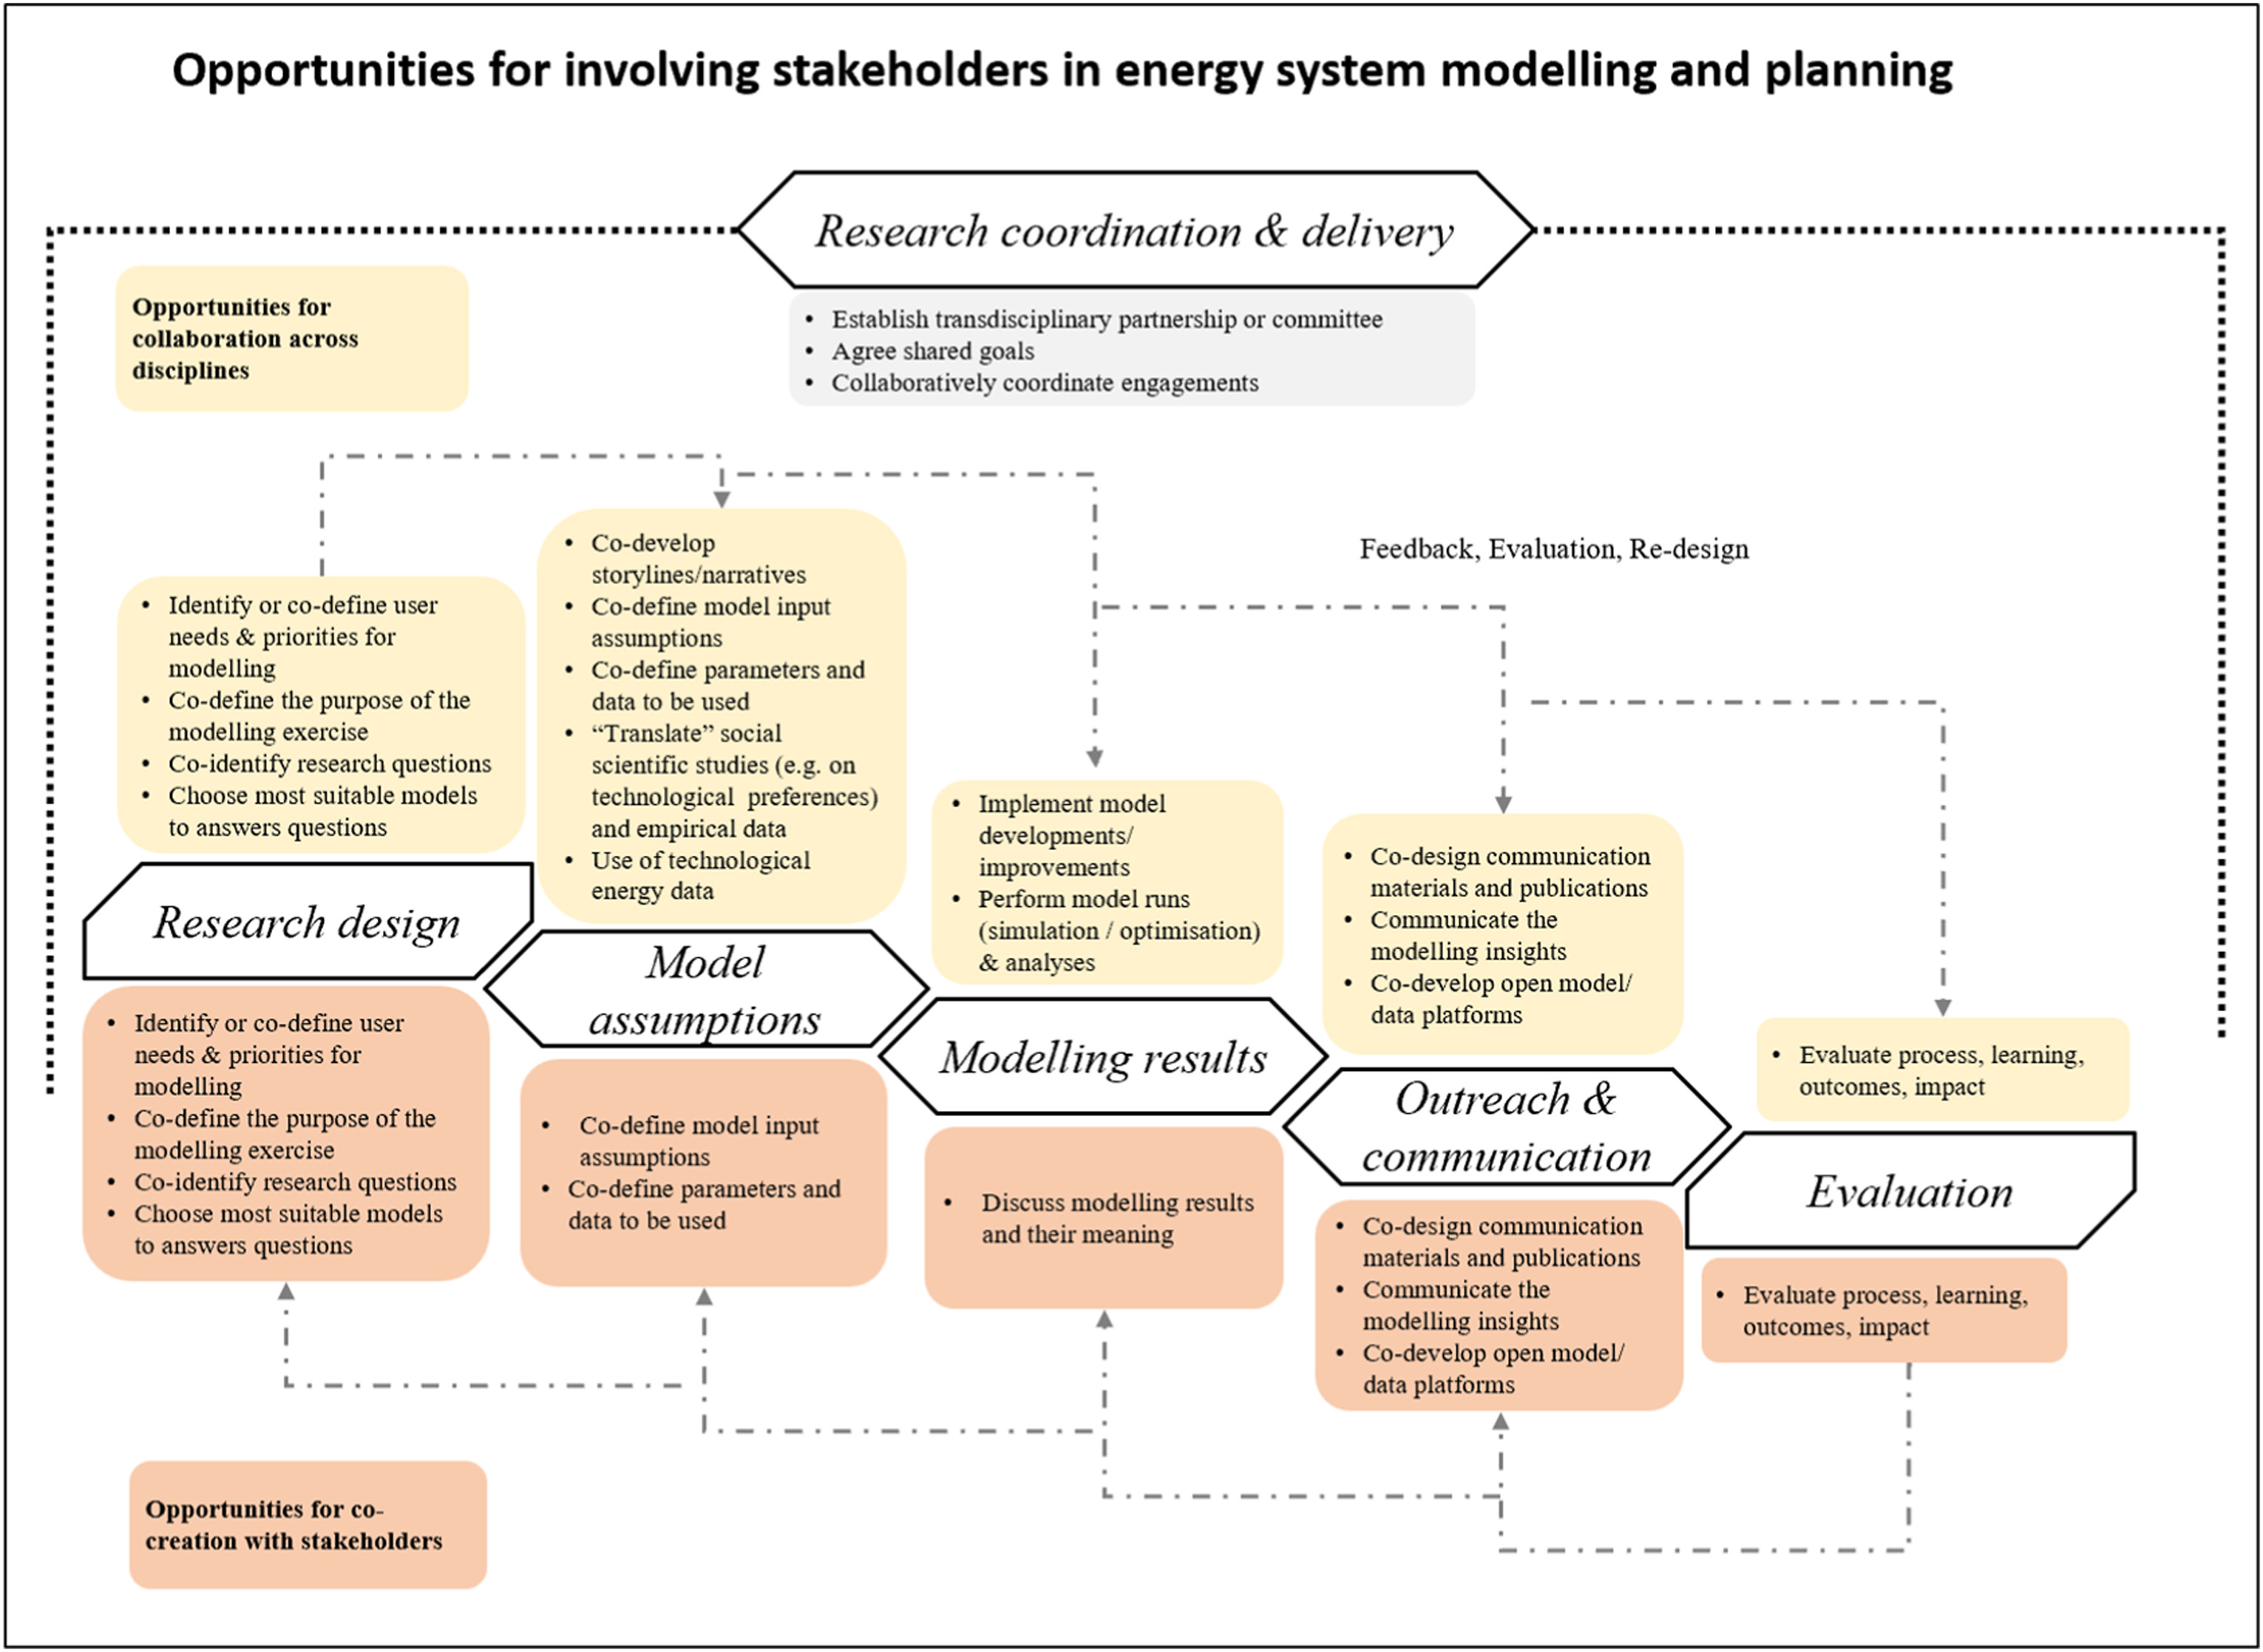
\includegraphics[width=\columnwidth]{figures/06_modeling_theory_chapter/participatory-modeling-flow-chart.jpg}
    \caption{Framework of opportunities for inter-/transdisciplinarity in energy
    systems modelling. Reproduced from \cite{mcgookin_advancing_2024}.}
    \label{fig:participatory-flow}
\end{figure}

\section{Modeling phases}
\label{section:modeling-phases}

\subsection{Pre-descriptive}

Link between normative and parametric uncertainties. Normative decisions (i.e.,
assumptions) are made about different model parameters. Along with which
technologies are represented. At this stage, the uncertainties addressed range
between aleatory and epistemic. The former is a ``known unknown'' that could be
improved with more research. The latter corresponds to ``unknown unknowns'' or a
``deep uncertainty'' that cannot be improved (cite).

Engagement with the public is still important, here, since addressing uncertain
parameters, such as technology costs, depends on your impression of the
underlying data distribution.


\subsection{Descriptive}
Link between parametric and structural. This is where the ``modeling'' happens.
Constraints and objectives give a model its descriptive power.

For example, in this phase it might be important to introduce specific
retirement schedules for power plants based on community feedback. Illinois
legislators included such a schedule in the \acf{ceja} to retire coal and gas
plants based on input from frontline communities in Illinois.

\subsection{Prescriptive}
Link between structural and normative. Model results are interpreted and policy
outcomes are prescribed. Alternatively, researchers may start the cycle anew by
using the model results to adjust the normative assumptions. Perhaps because the
model results don't show a desirable future?